% Numbers below are copied from results/summary/*.md (generated by scripts/aggregate.py);
% the tables are generated by scripts/make_tables.py.
\begin{table*}[!t]
\centering
\caption{Phase 2 (DL and hybrid) results at 250,000 events, mean$\pm$sd over 5 seeds. XGBoost repeated as the reference. Stack/Average are fit on the cal split, so post-hoc columns do not apply.}
\label{tab:dl_main}
\footnotesize
\setlength{\tabcolsep}{3.5pt}
\begin{tabular}{lcccccccc}
\toprule
Features & Model & ROC AUC & PR AUC & Brier & ECE & ECE$_\mathrm{Platt}$ & ECE$_\mathrm{iso}$ & Train s \\
\midrule
low (21) & XGBoost & 0.7376$\pm$0.0006 & 0.7481$\pm$0.0006 & 0.2064$\pm$0.0002 & 0.0053 & 0.0058 & 0.0072 & 5.1 \\
low (21) & MLP & 0.7601$\pm$0.0008 & 0.7685$\pm$0.0007 & 0.1992$\pm$0.0004 & 0.0312 & 0.0056 & 0.0086 & 21.4 \\
low (21) & Stack & \textbf{0.7655$\pm$0.0011} & 0.7740$\pm$0.0009 & 0.1960$\pm$0.0004 & 0.0057 & -- & -- & 26.5 \\
low (21) & Average & 0.7643$\pm$0.0011 & 0.7726$\pm$0.0009 & 0.1966$\pm$0.0005 & 0.0085 & -- & -- & 26.5 \\
geo (40) & XGBoost & 0.8011$\pm$0.0005 & 0.8111$\pm$0.0005 & 0.1812$\pm$0.0002 & 0.0037 & 0.0034 & 0.0081 & 11.6 \\
geo (40) & MLP & 0.8255$\pm$0.0006 & 0.8342$\pm$0.0005 & 0.1713$\pm$0.0003 & 0.0360 & 0.0033 & 0.0075 & 19.6 \\
geo (40) & Stack & \textbf{0.8307$\pm$0.0009} & 0.8397$\pm$0.0008 & 0.1672$\pm$0.0004 & 0.0032 & -- & -- & 31.2 \\
geo (40) & Average & 0.8291$\pm$0.0009 & 0.8376$\pm$0.0007 & 0.1682$\pm$0.0005 & 0.0100 & -- & -- & 31.2 \\
high (7) & XGBoost & 0.7872$\pm$0.0003 & 0.8050$\pm$0.0003 & 0.1872$\pm$0.0001 & 0.0062 & 0.0051 & 0.0065 & 1.5 \\
high (7) & MLP & 0.7930$\pm$0.0006 & 0.8109$\pm$0.0008 & 0.1848$\pm$0.0003 & 0.0051 & 0.0026 & 0.0066 & 19.4 \\
high (7) & Stack & \textbf{0.7934$\pm$0.0004} & 0.8112$\pm$0.0005 & 0.1845$\pm$0.0002 & 0.0024 & -- & -- & 20.9 \\
high (7) & Average & 0.7926$\pm$0.0002 & 0.8104$\pm$0.0003 & 0.1849$\pm$0.0001 & 0.0034 & -- & -- & 20.9 \\
all (28) & XGBoost & 0.8235$\pm$0.0006 & 0.8378$\pm$0.0005 & 0.1711$\pm$0.0003 & 0.0053 & 0.0061 & 0.0067 & 4.8 \\
all (28) & MLP & 0.8310$\pm$0.0007 & 0.8440$\pm$0.0006 & 0.1682$\pm$0.0006 & 0.0263 & 0.0030 & 0.0056 & 17.5 \\
all (28) & Stack & \textbf{0.8354$\pm$0.0006} & 0.8488$\pm$0.0005 & 0.1652$\pm$0.0003 & 0.0043 & -- & -- & 22.3 \\
all (28) & Average & 0.8351$\pm$0.0005 & 0.8485$\pm$0.0004 & 0.1654$\pm$0.0003 & 0.0049 & -- & -- & 22.3 \\
geo+high (47) & XGBoost & 0.8381$\pm$0.0003 & 0.8506$\pm$0.0004 & 0.1638$\pm$0.0001 & 0.0054 & 0.0053 & 0.0078 & 10.4 \\
geo+high (47) & MLP & 0.8422$\pm$0.0008 & 0.8531$\pm$0.0011 & 0.1632$\pm$0.0006 & 0.0362 & 0.0029 & 0.0061 & 17.0 \\
geo+high (47) & Wide\&Deep & 0.8330$\pm$0.0005 & 0.8418$\pm$0.0007 & 0.1671$\pm$0.0003 & 0.0284 & 0.0028 & 0.0068 & 21.8 \\
geo+high (47) & Stack & \textbf{0.8505$\pm$0.0003} & 0.8619$\pm$0.0005 & 0.1573$\pm$0.0002 & 0.0043 & -- & -- & 27.3 \\
geo+high (47) & Average & 0.8503$\pm$0.0004 & 0.8617$\pm$0.0005 & 0.1574$\pm$0.0002 & 0.0041 & -- & -- & 27.3 \\
\bottomrule
\end{tabular}
\end{table*}


\subsection{MLP versus tuned trees at a fixed budget (RQ4)}
At 250k events (Table~\ref{tab:dl_main}, five seeds; seed sd $\le$0.0008) the MLP beats tuned XGBoost
on every representation, and every comparison in Table~\ref{tab:comparisons} holds in all five seeds.
The margin depends on how much structure the inputs leave to be learned. It is largest on raw
measurements ($+0.023$ on \texttt{low}) and geometric features ($+0.024$ on \texttt{geo}), and
smallest on the 7 masses ($+0.006$ on \texttt{high}), where little interaction remains to discover.
The MLP also benefits from the symmetry-derived features ($+0.065$ over \texttt{low}), almost exactly
as much as XGBoost does ($+0.064$). Encoding the symmetry therefore helps the network too, and is
not just a work-around for axis-aligned splits.

\begin{table*}[!t]
\centering
\caption{Paired DeLong tests on the shared test set. $\Delta$AUC = A$-$B (mean$\pm$sd over seeds); last column: seeds in which the difference is significant at $\alpha=0.05$ in favour of A / B.}
\label{tab:comparisons}
\footnotesize
\setlength{\tabcolsep}{3.5pt}
\begin{tabular}{lllcc}
\toprule
Question & A & B & $\Delta$AUC & Sig. A/B \\
\midrule
DL vs trees on raw measurements & mlp|low & xgboost|low & 0.0226$\pm$0.0011 & 5/0 \\
DL vs trees on geometric features & mlp|geo & xgboost|geo & 0.0244$\pm$0.0006 & 5/0 \\
DL vs trees on raw + expert & mlp|all & xgboost|all & 0.0075$\pm$0.0005 & 5/0 \\
Feature engineering (geo) for trees & xgboost|geo & xgboost|low & 0.0635$\pm$0.0008 & 5/0 \\
Feature engineering (geo) for the MLP & mlp|geo & mlp|low & 0.0654$\pm$0.0010 & 5/0 \\
Geometry alone vs expert masses (MLP) & mlp|geo & mlp|high & 0.0325$\pm$0.0011 & 5/0 \\
Geometry alone vs expert masses (XGB) & xgboost|geo & xgboost|high & 0.0139$\pm$0.0004 & 5/0 \\
Geometry alone vs raw + expert (MLP) & mlp|geo & mlp|all & -0.0055$\pm$0.0011 & 0/5 \\
geo+expert vs raw+expert (MLP) & mlp|geo\_high & mlp|all & 0.0112$\pm$0.0012 & 5/0 \\
Hybrid 1: wide\&deep vs plain MLP, same inputs & widedeep|geo\_high & mlp|geo\_high & -0.0092$\pm$0.0008 & 0/5 \\
Hybrid 2: stacking vs MLP & stack|geo\_high & mlp|geo\_high & 0.0084$\pm$0.0008 & 5/0 \\
Hybrid 2: stacking vs XGB & stack|geo\_high & xgboost|geo\_high & 0.0124$\pm$0.0001 & 5/0 \\
Hybrid 2: learned stacking vs naive average & stack|geo\_high & average|geo\_high & 0.0002$\pm$0.0000 & 5/0 \\
Hybrid 2 on the paper's features: stacking vs MLP & stack|all & mlp|all & 0.0044$\pm$0.0005 & 5/0 \\
\bottomrule
\end{tabular}
\end{table*}


\subsection{Scaling with data}\label{sec:scaling}
\begin{table*}[!t]
\centering
\caption{Test ROC AUC vs data budget (train+val+cal events); mean$\pm$sd over seeds (3 seeds; 5 at 250k; 1 at 10.5M, \texttt{low}/\texttt{all} only).}
\label{tab:scaling}
\footnotesize
\setlength{\tabcolsep}{3.5pt}
\begin{tabular}{lccccc}
\toprule
Features & Model & 50k & 250k & 1M & 10.5M \\
\midrule
low (21) & LogReg & 0.5945$\pm$0.0003 & 0.5957$\pm$0.0001 & 0.5959$\pm$0.0000 & 0.5959 \\
low (21) & XGBoost & 0.6986$\pm$0.0011 & 0.7376$\pm$0.0006 & 0.7648$\pm$0.0012 & 0.8001 \\
low (21) & MLP & 0.7051$\pm$0.0018 & 0.7601$\pm$0.0008 & 0.8170$\pm$0.0005 & 0.8464 \\
geo (40) & LogReg & 0.6287$\pm$0.0004 & 0.6298$\pm$0.0001 & 0.6298$\pm$0.0001 & -- \\
geo (40) & XGBoost & 0.7618$\pm$0.0018 & 0.8011$\pm$0.0005 & 0.8230$\pm$0.0005 & -- \\
geo (40) & MLP & 0.7572$\pm$0.0044 & 0.8255$\pm$0.0006 & 0.8594$\pm$0.0002 & -- \\
all (28) & LogReg & 0.6835$\pm$0.0006 & 0.6842$\pm$0.0002 & 0.6842$\pm$0.0001 & 0.6844 \\
all (28) & XGBoost & 0.8073$\pm$0.0007 & 0.8235$\pm$0.0006 & 0.8365$\pm$0.0001 & 0.8507 \\
all (28) & MLP & 0.7858$\pm$0.0005 & 0.8310$\pm$0.0007 & 0.8519$\pm$0.0001 & 0.8680 \\
geo+high (47) & LogReg & 0.6908$\pm$0.0003 & 0.6918$\pm$0.0002 & 0.6918$\pm$0.0001 & -- \\
geo+high (47) & XGBoost & 0.8180$\pm$0.0005 & 0.8381$\pm$0.0003 & 0.8528$\pm$0.0003 & -- \\
geo+high (47) & MLP & 0.7909$\pm$0.0006 & 0.8422$\pm$0.0008 & 0.8688$\pm$0.0001 & -- \\
\bottomrule
\end{tabular}
\end{table*}

\begin{figure*}[!t]
\centering
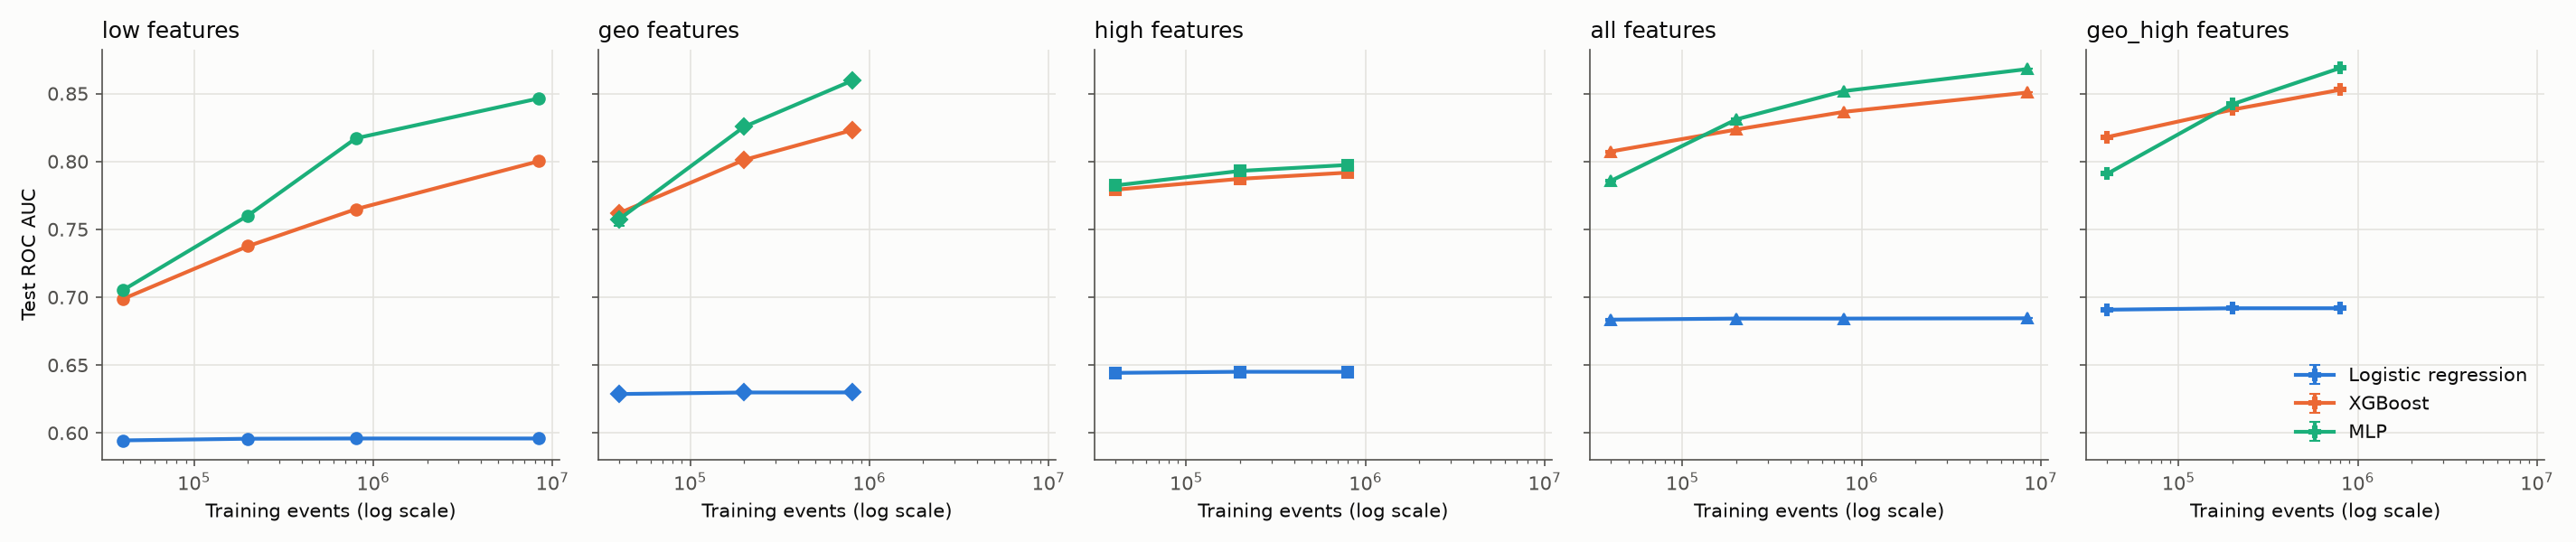
\includegraphics[width=\textwidth]{scaling.png}
\caption{Test ROC AUC vs training events (log scale), mean$\pm$sd over seeds. On the richer
representations (\texttt{geo}, \texttt{all}, \texttt{geo+high}) XGBoost (orange) leads at 50k events
and the MLP (green) overtakes it by 250k. On \texttt{low} the MLP leads at every budget and pulls away
with more data. The 7-mass set (\texttt{high}) saturates for both models.}
\label{fig:scaling}
\end{figure*}
The ranking at 250k is not universal (Table~\ref{tab:scaling}, Fig.~\ref{fig:scaling}). At
\textbf{50k events XGBoost is better} on the richer representations: \texttt{all} (0.807 vs.\ 0.786),
\texttt{geo+high} (0.818 vs.\ 0.791) and \texttt{geo} (0.762 vs.\ 0.757). The MLP is only narrowly
ahead on \texttt{low} ($+0.007$) and \texttt{high} ($+0.003$). The crossover lies between 50k and
250k, and the MLP's lead grows steadily after that. On \texttt{low} it is $+0.007$ at 50k, $+0.023$ at
250k, $+0.052$ at 1M and $+0.046$ at 10.5M.
At 1M events the MLP on geometry alone \emph{overtakes} the MLP on the paper's raw+expert features
(0.859 vs.\ 0.852, all three seeds), a reversal of the 250k result ($-0.006$). With enough data, the
symmetry-derived representation carries more usable information than the masses.

On the full 10.5M pool, the MLP on the 21 raw measurements reaches 0.846, within 0.005 of XGBoost
given the expert features (0.851). The MLP on \texttt{all} reaches 0.868. This reproduces the central
claim of Baldi \emph{et al.} \cite{baldi2014searching}: with enough data, a network on raw
measurements nearly matches tree ensembles that have the expert features. Their deeper network,
trained for much longer, reached higher absolute values (0.88 on \texttt{all}). Ours stopped at the
50-epoch cap while still improving, so these numbers are lower bounds.

\subsection{Calibration}
The MLP ranks better but is less calibrated. Its raw ECE is 0.026--0.036 on every representation
except \texttt{high} (0.005), five to seven times XGBoost's. Platt scaling on the cal split repairs
it, to 0.003--0.006, without changing the AUC (Table~\ref{tab:dl_main}). Isotonic regression is slightly
worse (0.006), as expected with 25k calibration events. This matches Guo \emph{et al.}'s observation
for modern networks \cite{guo2017calibration}. Here the cause is early stopping on AUC rather than
on log loss, combined with batch-statistics noise.

\subsection{Ablations (RQ5)}\label{sec:ablations}
\begin{table*}[!t]
\centering
\caption{MLP ablations (3 seeds, 250,000 events): test ROC AUC and change vs the baseline (3$\times$256, ReLU, BatchNorm, dropout 0.1, Glorot init).}
\label{tab:ablations}
\footnotesize
\setlength{\tabcolsep}{3.5pt}
\begin{tabular}{lcccccc}
\toprule
Variant & AUC (low) & $\Delta$ & AUC (all) & $\Delta$ & Params & Epochs \\
\midrule
baseline & 0.7605$\pm$0.0009 & +0.0000 & 0.8314$\pm$0.0005 & +0.0000 & 139,009 & 39 \\
no\_batchnorm & 0.7563$\pm$0.0007 & -0.0041 & 0.8265$\pm$0.0013 & -0.0048 & 137,473 & 33 \\
no\_dropout & 0.7394$\pm$0.0016 & -0.0211 & 0.8125$\pm$0.0013 & -0.0188 & 139,009 & 17 \\
dropout\_0.3 & 0.7642$\pm$0.0008 & +0.0037 & 0.8337$\pm$0.0005 & +0.0023 & 139,009 & 50 \\
no\_weight\_decay & 0.7592$\pm$0.0004 & -0.0013 & 0.8310$\pm$0.0003 & -0.0004 & 139,009 & 38 \\
default\_init & 0.7585$\pm$0.0007 & -0.0020 & 0.8313$\pm$0.0006 & -0.0001 & 139,009 & 35 \\
default\_init\_no\_bn & 0.7546$\pm$0.0006 & -0.0059 & 0.8266$\pm$0.0004 & -0.0048 & 137,473 & 32 \\
tanh\_no\_bn\_xavier & 0.7532$\pm$0.0008 & -0.0073 & 0.8307$\pm$0.0005 & -0.0007 & 137,473 & 48 \\
tanh\_no\_bn\_default\_init & 0.7554$\pm$0.0006 & -0.0051 & 0.8304$\pm$0.0003 & -0.0010 & 137,473 & 48 \\
depth\_1 & 0.7250$\pm$0.0015 & -0.0355 & 0.8068$\pm$0.0008 & -0.0246 & 6,401 & 50 \\
depth\_5 & 0.7608$\pm$0.0005 & +0.0003 & 0.8306$\pm$0.0008 & -0.0008 & 271,617 & 34 \\
width\_64 & 0.7498$\pm$0.0009 & -0.0107 & 0.8256$\pm$0.0011 & -0.0058 & 10,177 & 50 \\
width\_512 & 0.7592$\pm$0.0021 & -0.0013 & 0.8283$\pm$0.0014 & -0.0031 & 540,161 & 28 \\
\bottomrule
\end{tabular}
\end{table*}

\begin{figure*}[!t]
\centering
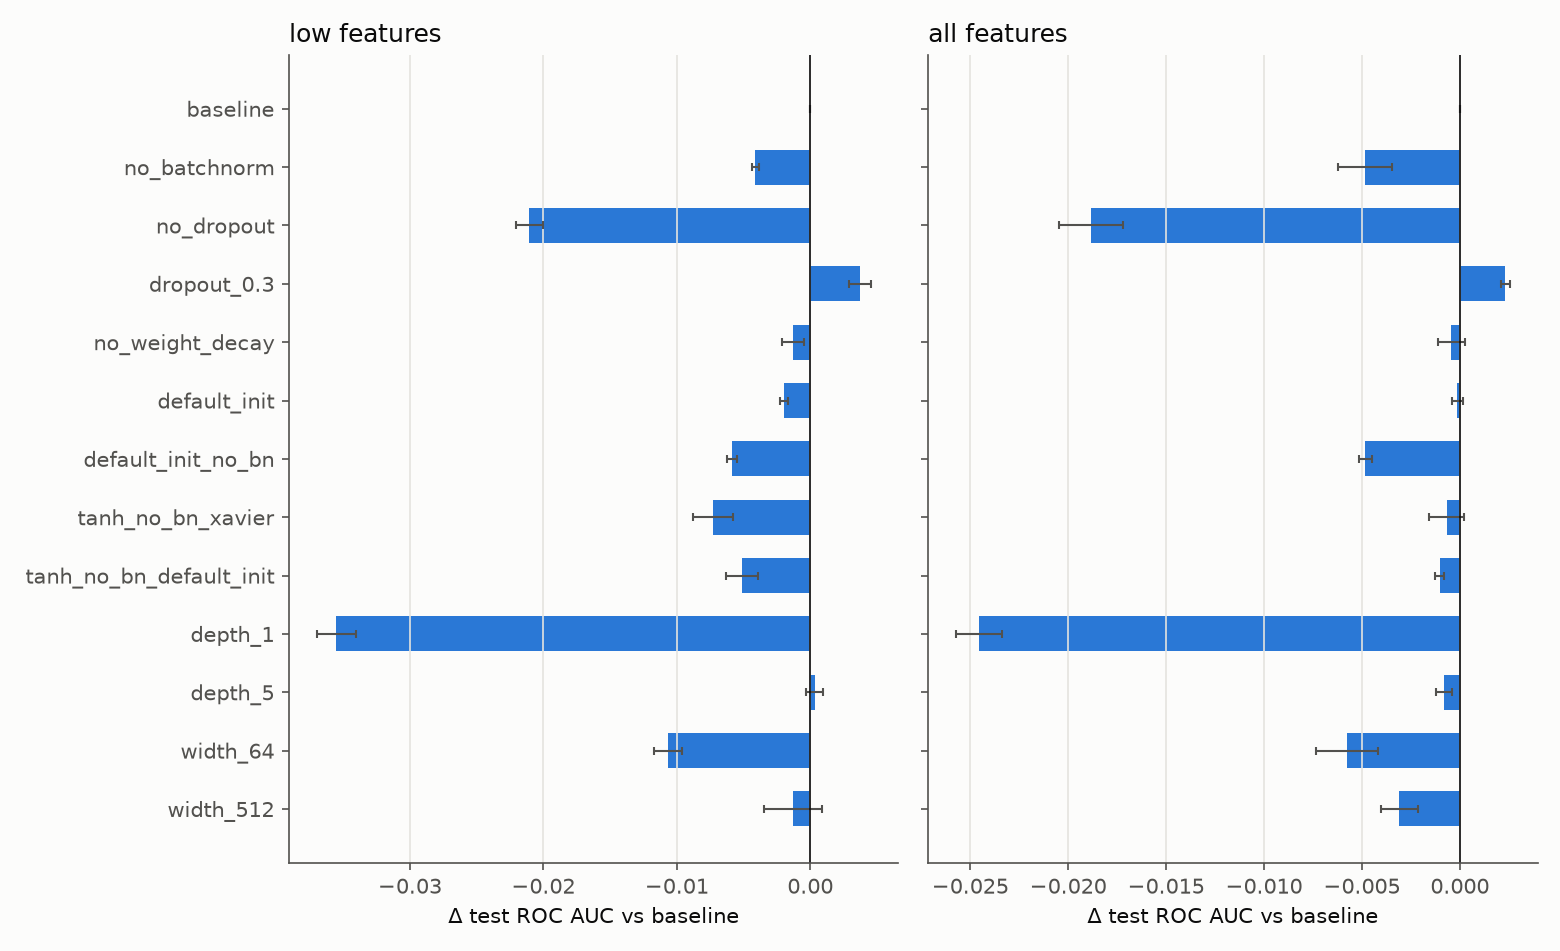
\includegraphics[width=0.49\textwidth]{ablation_auc.png}\hfill
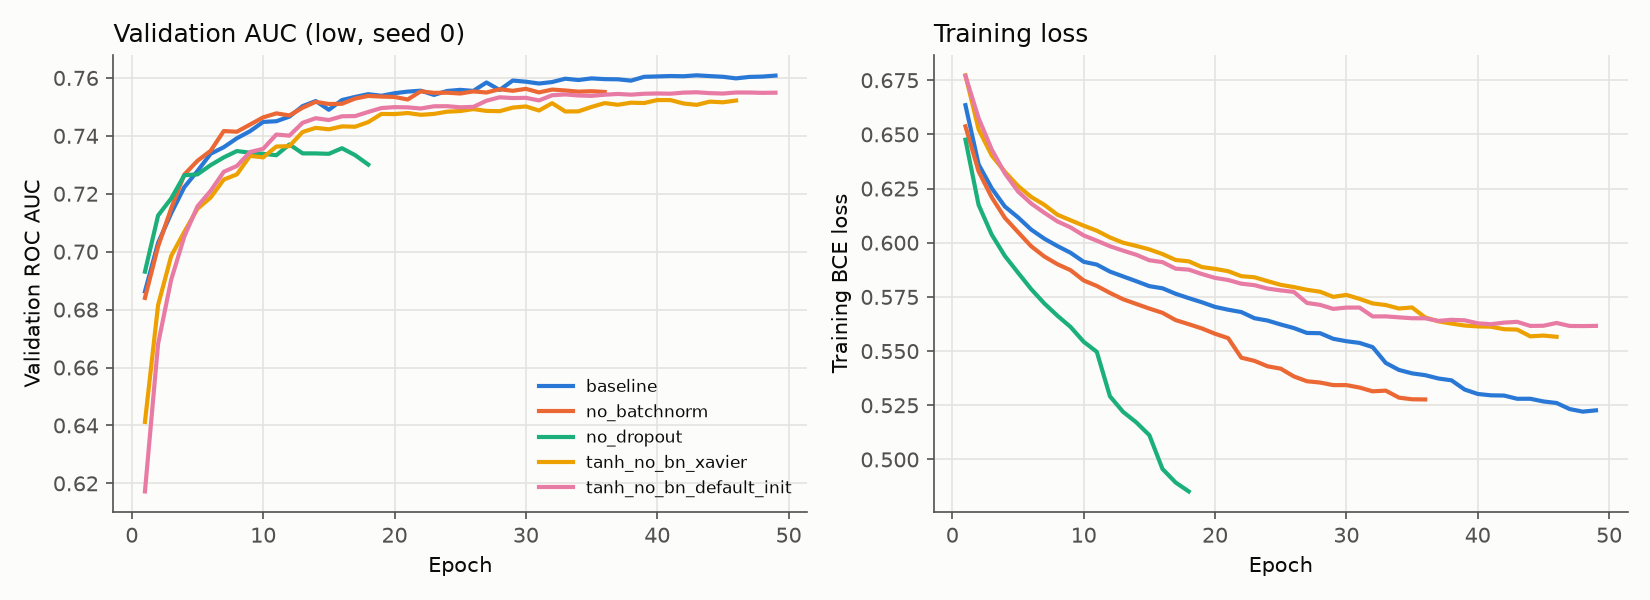
\includegraphics[width=0.49\textwidth]{learning_curves.png}
\caption{Left: change in test ROC AUC vs the baseline MLP (mean$\pm$sd, 3 seeds). Right: validation
AUC and training loss per epoch (\texttt{low}, seed~0). Without dropout the training loss collapses
while validation AUC peaks near epoch 12 and then declines: classic overfitting.}
\label{fig:ablation}
\end{figure*}
Table~\ref{tab:ablations} and Fig.~\ref{fig:ablation} change one design choice at a time (sd
$\approx$0.001).
\begin{itemize}
\item \textbf{Depth matters most.} One hidden layer loses 0.036 on \texttt{low} and 0.025 on
\texttt{all}. This is the shallow-network deficit Baldi \emph{et al.} reported. Five layers neither
help nor hurt at this budget.
\item \textbf{Dropout is the key regulariser.} Removing it costs 0.021, and the learning curves show
overfitting from about epoch 12. Raising it to 0.3 \emph{improves} the baseline by $+0.004$/$+0.002$,
and that run hit the 50-epoch cap still improving. Our baseline was therefore under-regularised. We
report this as a finding rather than retroactively retuning on test-scored results.
\item \textbf{Capacity.} Width 64 costs 0.011 on \texttt{low}, and width 512 adds nothing.
\item \textbf{BatchNorm} adds a modest 0.004--0.005.
\item \textbf{Initialisation.} With BatchNorm, Glorot vs.\ PyTorch's default initialisation is
immaterial ($\le$0.002), as the theory in Section~\ref{sec:theory} predicts. Without BatchNorm,
default initialisation loses a little more than Glorot (ReLU: $-0.006$ vs.\ $-0.004$). In the
tanh/no-BatchNorm setting that Glorot and Bengio studied, however, Glorot initialisation is
\emph{not} better at depth~3 ($-0.007$ vs.\ $-0.005$). Their vanishing-gradient effect appears in
deeper networks trained with plain SGD. Adam's per-parameter step sizes largely compensate for a
mis-scaled initialisation in a 3-layer network.
\end{itemize}

\subsection{Hybrid approach (RQ6)}
\textbf{Hybrid 1, wide \& deep: a negative result.} Routing the 7 masses around the deep tower
\emph{lowers} the AUC relative to a plain MLP on exactly the same 47 inputs: $-0.009$ at 250k and
$-0.006$ at 1M, significant in every seed. The plain MLP already learns to use the masses where they
help. Isolating them in a 32-unit side path reduces the tower's ability to combine masses with
geometry, and the combination is where the gain lies (\texttt{geo+high} beats both
\texttt{geo} and \texttt{high}). We keep this experiment because it tests a specific, physically
motivated hypothesis against a matched control, and the answer is informative: expert features help
most as \emph{inputs to be mixed}, not as a separate path.

\textbf{Hybrid 2, stacking: a positive result.} The logistic stack of XGBoost and the MLP beats
\emph{both} of its base models at every budget (50k--10.5M) and on every feature set. It is the best
model overall at 250k and 1M; at 50k plain averaging ties it to within 0.0003. On \texttt{geo+high}
at 250k it reaches
\textbf{0.851}, against 0.842 for the MLP and 0.838 for XGBoost ($+0.008$ and $+0.012$, all seeds),
with an ECE of 0.004 and no post-hoc step. On the paper's \texttt{all} features it adds $+0.004$ over
the MLP. Plain averaging achieves almost the same ranking (within 0.0002 at 250k and 0.0017 at 1M).
The ranking gain therefore comes from combining two models with different inductive biases, and the
learned meta-learner contributes calibration and adaptivity. Its weights show this adaptivity. At
250k it weights the two models comparably ($\beta_\mathrm{XGB}\approx0.5$,
$\beta_\mathrm{MLP}\approx0.45$ on \texttt{geo+high}). At 1M the weights shift to 0.30 and 0.68. On
the full pool they are 0.15 and 0.91. As the MLP improves with data, the stacker learns to trust it,
and the hybrid's advantage shrinks to $+0.0003$ at 10.5M.
